\documentclass{beamer}
\usepackage{amsmath}
\usepackage{subfig}
\usepackage[backend=biber, style=authoryear]{biblatex}
\addbibresource{references.bib}
\usetheme{Antibes}
\title{Answering to why-not questions in group recommendations}
\author{Noora Pöysti \& Väinö-Waltteri Granat}

\begin{document}
\frame{\titlepage}


\begin{frame}
    \frametitle{Basic idea}
    This presentation shows how we have implemented answers to why-not questions.
\end{frame}

\begin{frame}
    \frametitle{Granularity case - Atomic}
    For atomic why-not questions we decided to use general answers to respond, such as "item does not exists", "tie break", "too few items asked". 

\end{frame}

\begin{frame}
  \frametitle{Granularity case - Group}

  Our answers are based on the likelyhood of a movie beloning to certain genre, begin included among the groups top 20 movies.
  
  If group has watched a lot of dramas but only a few westerns it is highly likely that the top 20 movies include
   more dramas than westerns. (Assuming the the users like dramas and westerns equally)

  \begin{align*}
    & N = \text{Number of movies seen by group} \\
    & N_g = \text{number of movies of particular genre seen by group} \\
    & P(A) = \text{Likelyhood of why-not genre belonging to top 20 movies }\\
  & P(A) = 1-P(\overline{A}) = 1 - \frac{{N-N_g \choose 20}}{{N \choose 20}} \\
  \end{align*} 
\end{frame}

\begin{frame}
  \frametitle{Group histogram}
  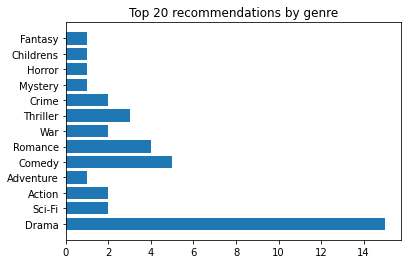
\includegraphics[width=\textwidth]{genre_top20.png}
\end{frame}

\begin{frame}
  \frametitle{Group histograms}
  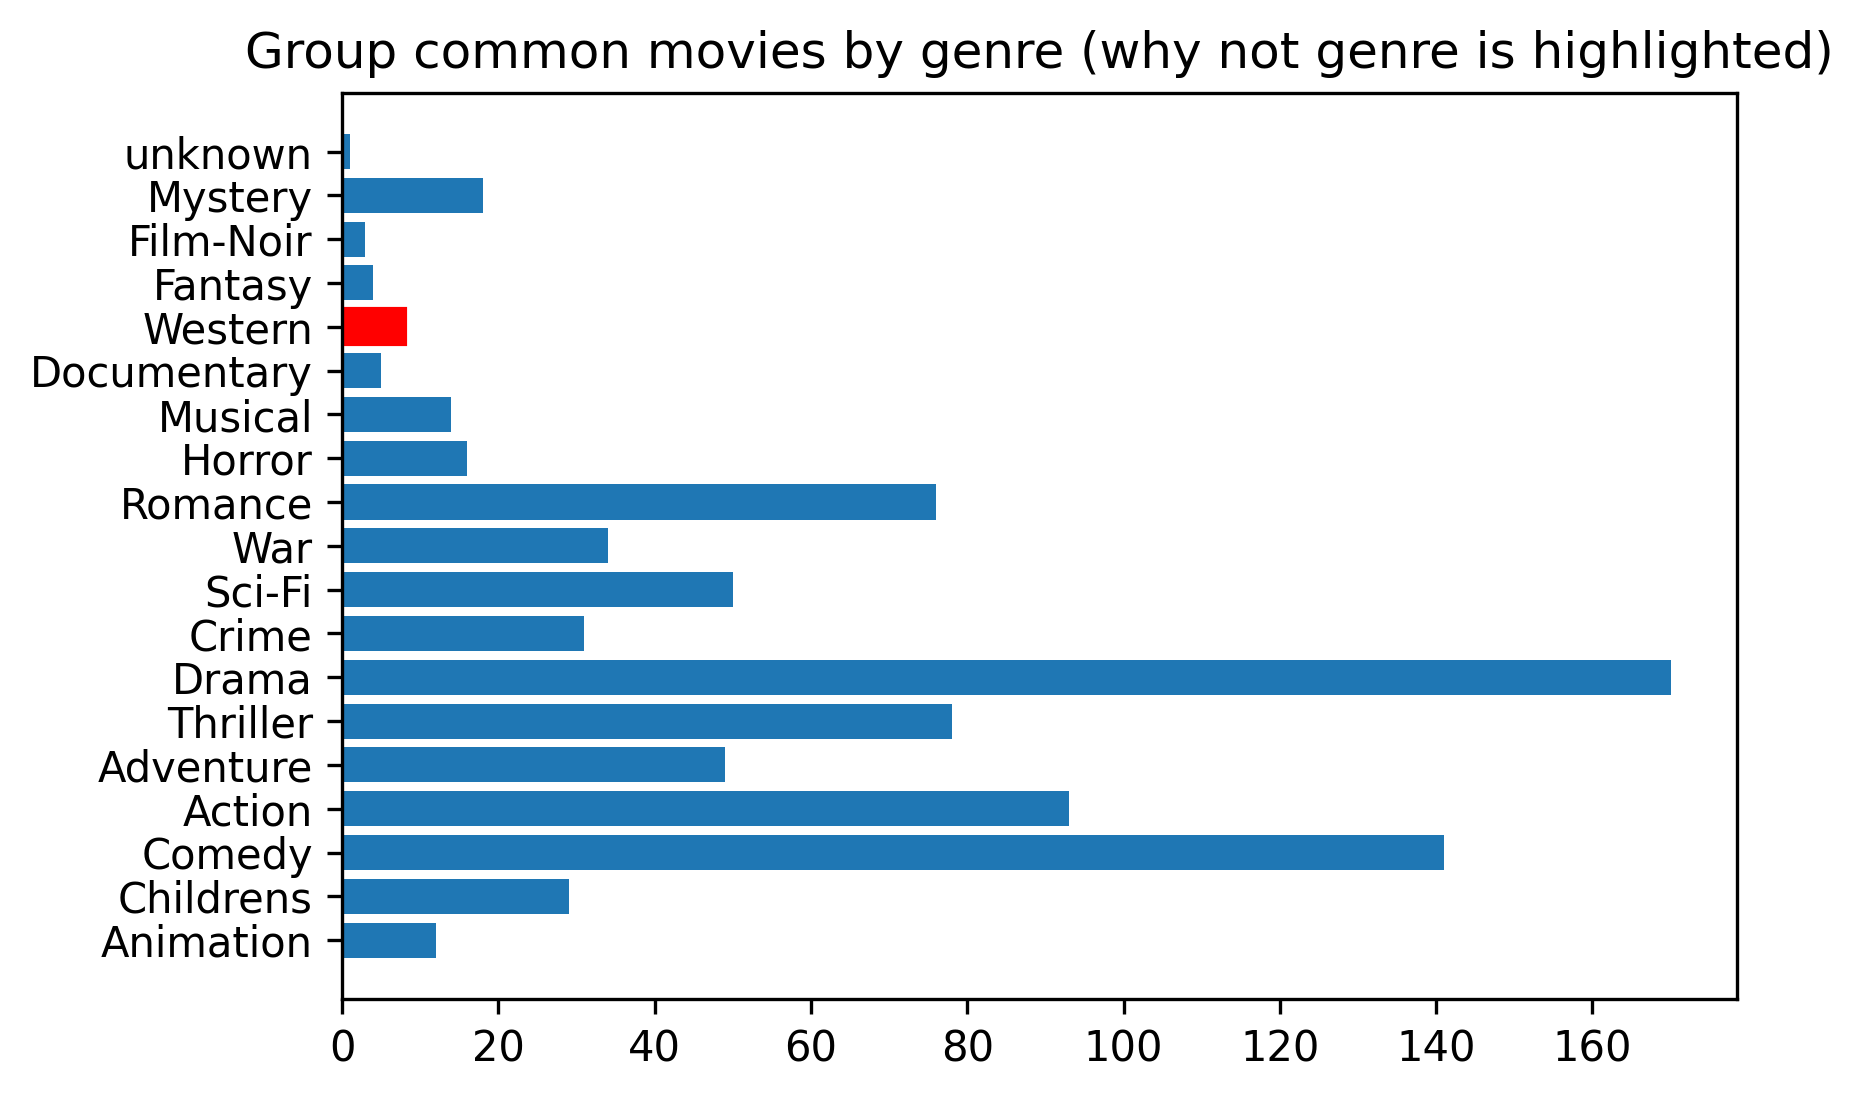
\includegraphics[width=\textwidth]{genre_moviesbygenre.png}
\end{frame}


\begin{frame}
  \frametitle{Group - most highly rated movies per genre}
  Other way we answer why-not guestions for groups is by looking at most highly rated movies for the group in each genre.
  Since we known the threshold that was needed to be included in the top 20 list, we can say when users haven't rated the movies
  of the given genre as highly as was needed to exceed that treshold.
  
\end{frame}

\begin{frame}
  \frametitle{Rating tresholds}
  \begin{center}
  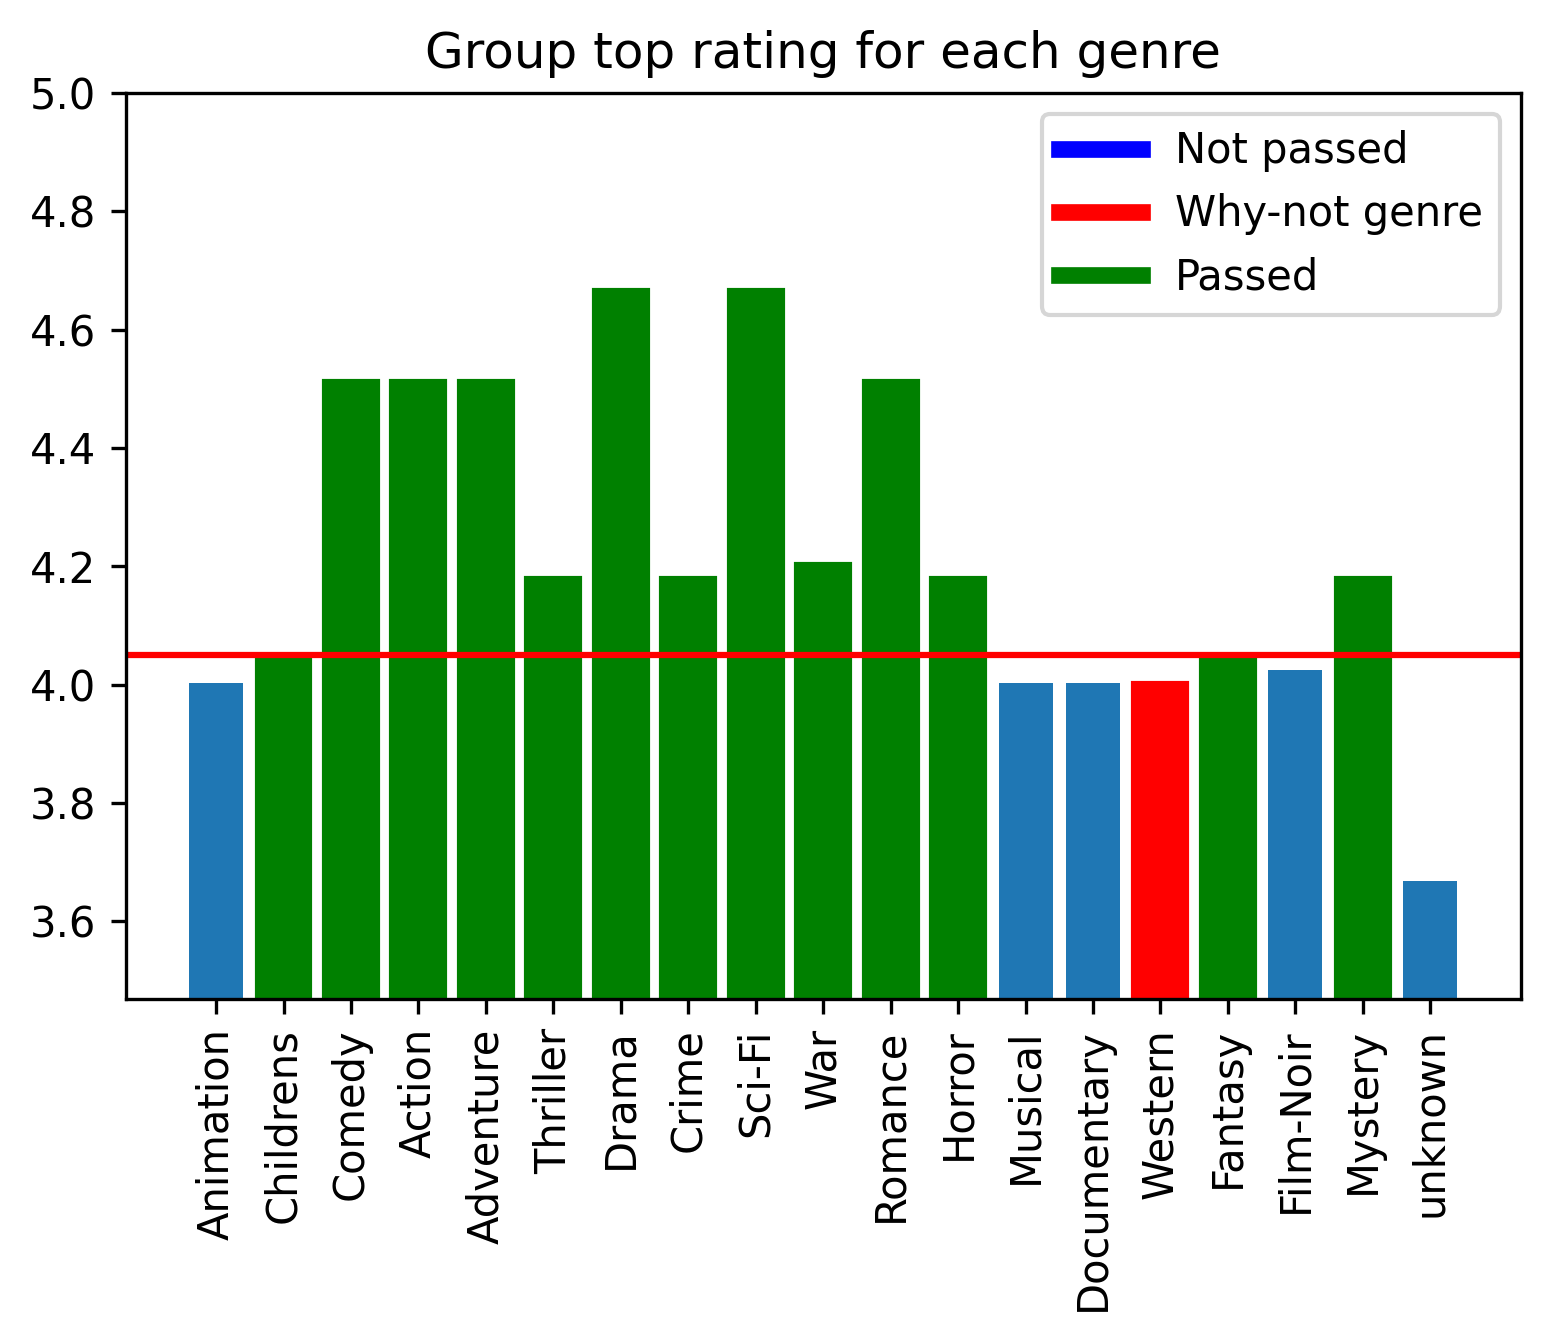
\includegraphics[height=0.85\textheight]{genre_toprating.png}
  \end{center}
\end{frame}


\begin{frame}
  \frametitle{Absenteeism}
  We answer absenteeism case by comparing item $i$ in question with the corresponding 
  item $j$ at wanted position $pos$ as defined in the why-not question. Our function takes
  an item $i$ for which we want to know why it is not in position $pos$. The function then tells
  how many positions the item $i$ was behind the item in position $pos$. 
\end{frame}

\begin{frame}
  \frametitle{Absenteeism}
  We also compare items $i$ and $j$ in terms of how the users of the given group have rated
  them.
\end{frame}


\begin{frame}
  \frametitle{Absenteeism - Item comparison}
  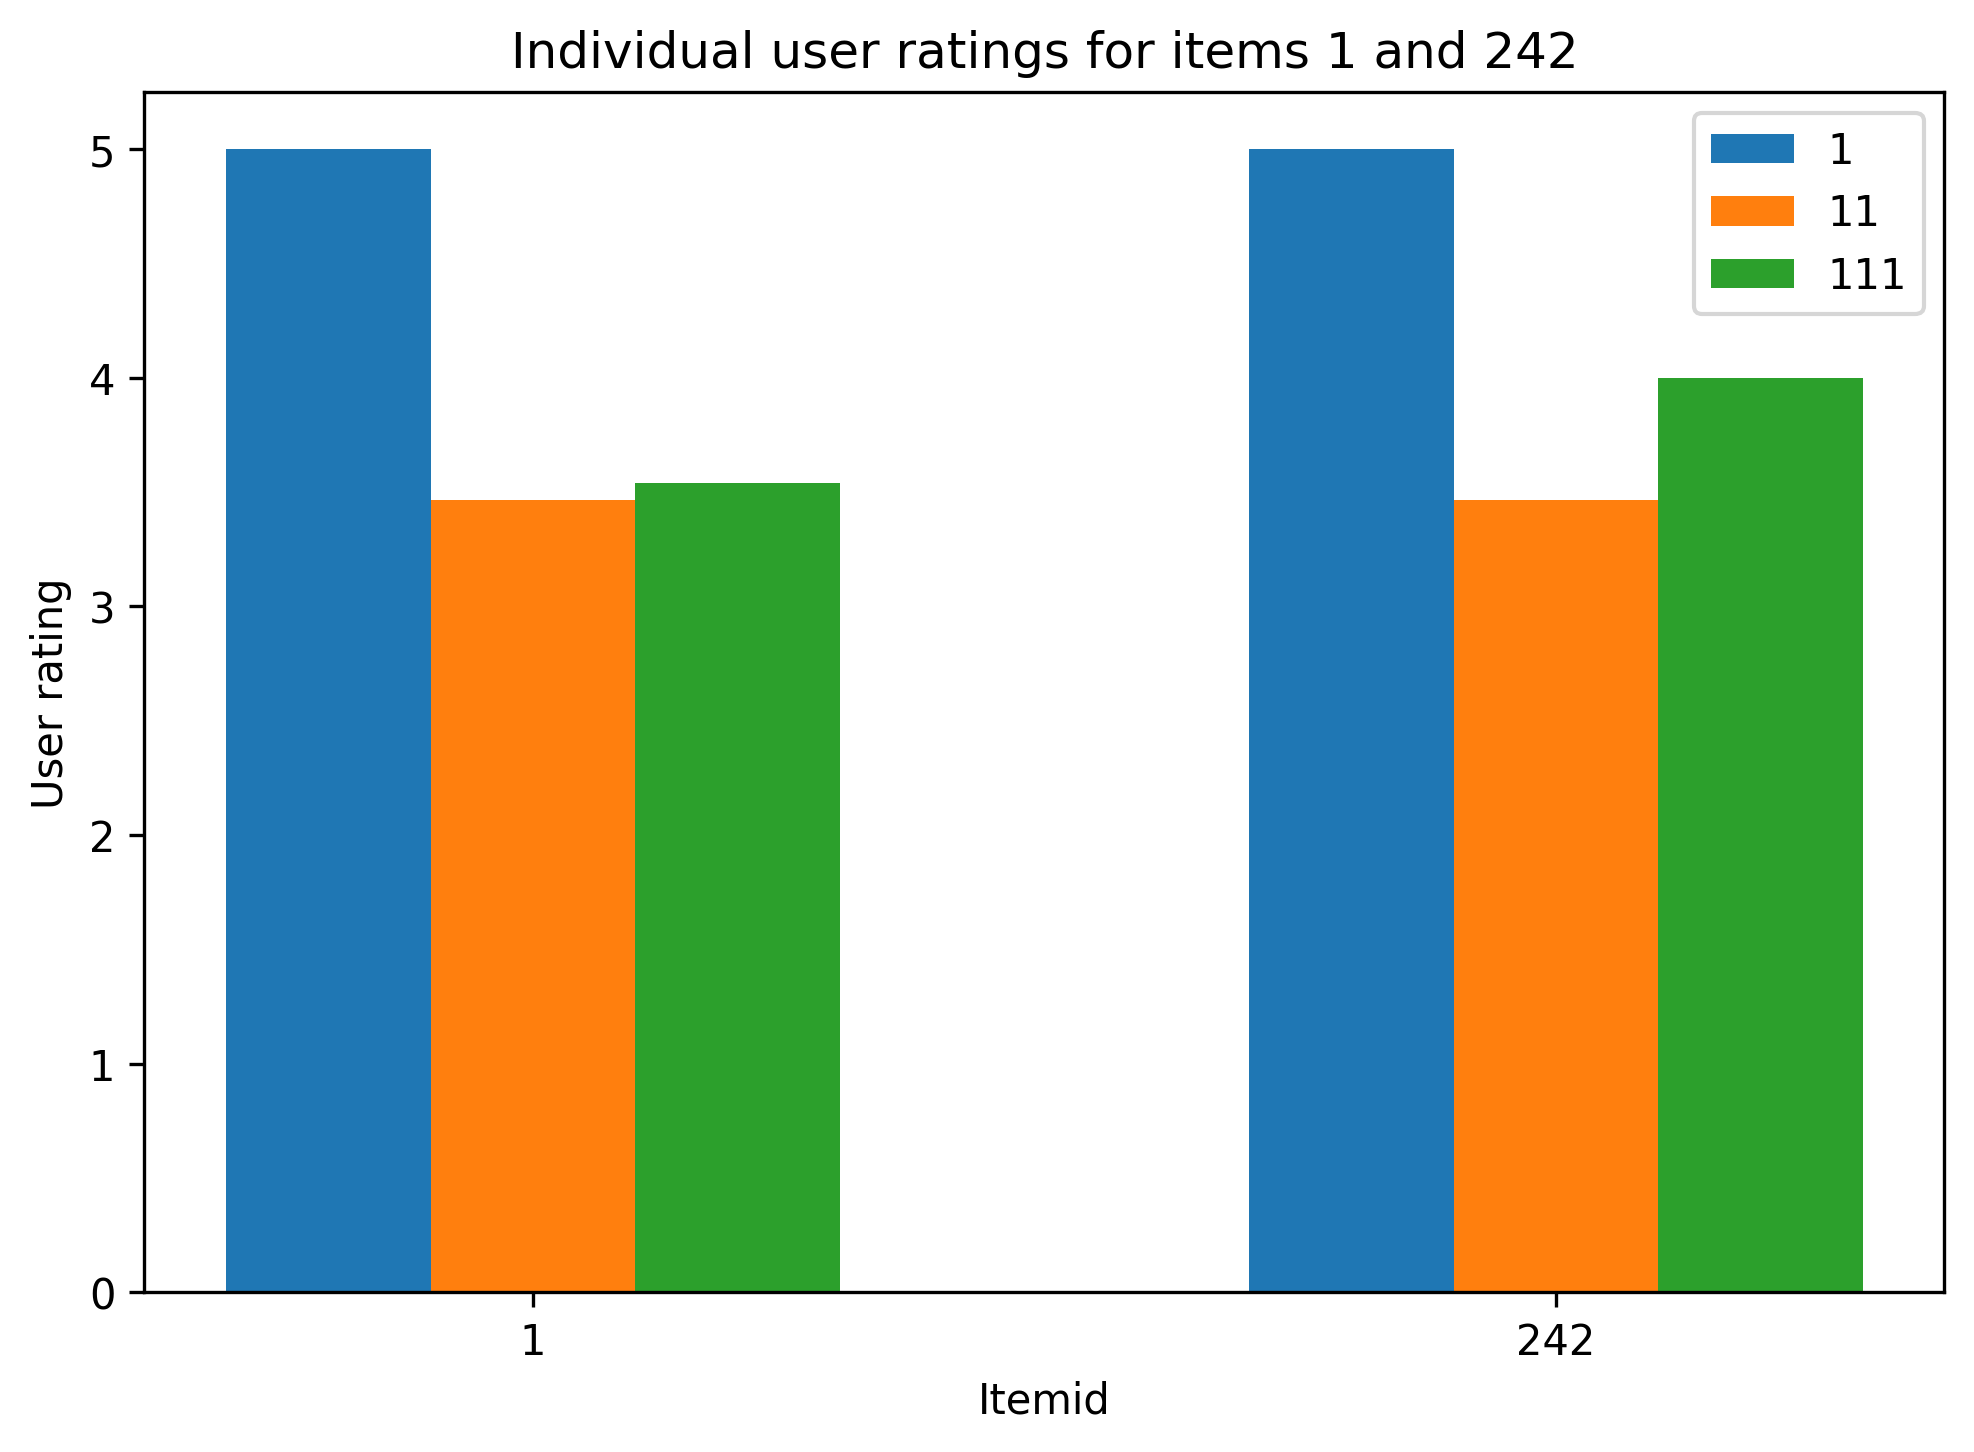
\includegraphics[width=0.9\textwidth]{abs_ratings.png}
\end{frame}



\end{document}
